%% Copernicus Publications Manuscript Preparation Template for LaTeX Submissions

\documentclass[journal abbreviation, npg]{copernicus}

\begin{document}

\linenumbers

\title{Estimation of the total magnetization direction of approximately spherical bodies}

\author[1]{D. ~P. ~Sales}
\author[1]{V. ~C. ~Oliveira Jr.}
\author[1]{V. ~C. ~F. ~Barbosa}
\author[1, 2]{L. ~Uieda}

\affil[1]{Observat\'orio Nacional, Brazil}
\affil[2]{Universidade do Estado do Rio de Janeiro, Brazil}

%% The [] brackets identify the author to the corresponding affiliation, 1, 2, 3, etc. should be inserted.

\runningtitle{Magnetization direction of spherical bodies}

\runningauthor{D. P. Sales et al.}

\correspondence{V. C. Oliveira Jr. \\ (vandscoelho@gmail.com)}

\received{}
\pubdiscuss{} %% only important for two-stage journals
\revised{}
\accepted{}
\published{}

%% These dates will be inserted by the Publication Production Office during the typesetting process.

\firstpage{1}

\maketitle  %% Please note that for the copernicus2.cls this command needs to be inserted after \abstract{TEXT}

\begin{abstract}
TEXT
\end{abstract}

\section{Introduction}
TEXT

\section{Methodology}

\subsection{Parameterization and Forward Problem}

Let $\vec{\Delta T}^{o}$ be the observed data vector, whose $i$th element $\Delta T^{o}_{i}$, $i = 1, ..., N$, is the total field anomaly measured at the position $(x_{i}, y_{i}, z_{i})$ (black dots in Fig. \ref{fig:geometric-aspects}). In this Cartesian coordinate system, $x$ points to geographic North, $y$ points to East and $z$ points downward. In general, the total field anomaly is produced by a magnetized  susceptibility distribution which is anomalous with respect to the mean susceptibility of the crust. Mathematically, $\Delta T^{o}_{i}$ can be written as
\begin{equation}
\Delta T^{o}_{i} = \Vert \vec{T}_i \Vert + \Vert \vec{F}_i \Vert \: ,
\label{eq:tfanomaly-i}
\end{equation}
where $\Vert \Vert$ indicates the Euclidean norm, $\vec{F}_i$ is the Geomagnetic field vector and $\vec{T}_i$ is the Total Field, both at $(x_{i}, y_{i}, z_{i})$. The Total Field vector can be represented by the sum
\begin{equation}
\vec{T}_i = \vec{F}_i + \vec{B}_i \: ,
\label{eq:tfvector-i}
\end{equation}
where $\vec{B}_i$ is the Total Magnetic Induction vector produced by all magnetic sources (magnetized anomalous susceptibility distribution) at the position $(x_{i}, y_{i}, z_{i})$ \citep{blakely1996, langel-hinze1998}.

For local or regional scale magnetic studies, it is very common to consider that (i) the Geomagnetic Field $\vec{F}_i$ (Eq. \ref{eq:tfanomaly-i}) is a constant vector $\vec{F}_{0}$ throughout the study area and (ii) that $\Vert \vec{F}_{0} \Vert \gg \Vert \vec{B}_{i} \Vert$, $i = 1, ..., N$ \citep{telford-etal1990, blakely1996}. The second assumption is equivalent to say that the Total Magnetic Induction $\vec{B}_i$ (Eq. \ref{eq:tfanomaly-i}) is a small perturbation of the Geomagnetic field throughout the study area. These two assumptions make possible to approximate the Euclidean norm of the Total Field vector $\vec{T}_i$ (Eq. \ref{eq:tfanomaly-i}) by a first-order Taylor's expansion as follows
\begin{equation}
\begin{array}{cl}
\Vert \vec{T}_{i} \Vert & 
\approx \Vert \vec{F}_{0} + \vec{B}_{i} \Vert \\
\: &
\approx \Vert \vec{F}_{0} \Vert + \hat{\vec{F}}^{\intercal}\vec{B}_{i} \: ,
\end{array}
\label{eq:total-field-app}
\end{equation}
where $^{\intercal}$ indicates transposition and
\begin{equation}
\hat{\vec{F}} = \dfrac{\vec{F}_{0}}{\Vert \vec{F}_{0} \Vert}
\label{eq:unit-vector}
\end{equation}
is a unit vector (with the same direction of the Geomagnetic field) representing the gradient of the function $\Vert \vec{T}_{i} \Vert$ with respect to the components of the vector $\vec{T}_{i}$ \citep{blakely1996}. By introducing this first-order Taylor's expansion into the total field magnetic anomaly (Eq. \ref{eq:tfanomaly-i}), we obtain an approximated total field anomaly given by
\begin{equation}
\Delta T_{i} \approx \hat{\vec{F}}^{\intercal}\vec{B}_{i} \: , \qquad i = 1, ..., N \: .
\label{eq:approx-tfanomaly-i}
\end{equation}

Lets consider that the magnetic sources can be represented by a set of $L$ uniformly magnetized spheres. In this case, the Total Magnetic Induction $\vec{B}_i$ is given by
\begin{equation}
\vec{B}_i = \sum_{j = 1}^{L} \vec{b}_{i}^{j} \: ,
\label{eq:total-induction-i}
\end{equation}
being $\vec{b}^{j}_{i}$ the magnetic induction produced, at the position $(x_{i}, y_{i}, z_{i})$, by the $j$th sphere, $j = 1, ..., L$, with radius $R_ {j}$ (dashed straight lines in Fig. \ref{fig:geometric-aspects}), centre at $(xc_{j}, yc_{j}, zc_{j})$ (grey dots in Fig. \ref{fig:geometric-aspects}) and magnetization vector $\vec{m}^{j}$ given by
\begin{equation}
\vec{m}^{j} =
\left[
\begin{array}{c}
mx_{j} \\
my_{j} \\
mz_{j}
\end{array}
\right]_ {3 \times 1} \: .
\label{eq:mag-vector-j}
\end{equation}
The magnetic induction $\vec{b}^{j}_{i}$ can be written as
\begin{equation}
\vec{b}^{j}_{i} = C_{m} \: \mathbf{M}_{i}^{j} \: 
                  \dfrac{4}{3} \pi R_{j}^{3} \:
                  \vec{m}^{j} \: ,
\label{eq:j-induction-i}
\end{equation}
where $C_{m}$ is a constant given by $\mu_{0} / {4 \pi}=10^{-7}$ $\frac{H}{m}$, $\mu_{0}$ is the vacuum permeability and $\mathbf{M}_{i}^{j}$ is the matrix 
\begin{equation}
\mathbf{M}^{j}_{i} =
\left[
\begin{array}{ccc}
\frac{\partial^{2}}{\partial x \partial x} \frac{1}{r_{j}} &
\frac{\partial^{2}}{\partial x \partial y} \frac{1}{r_{j}} &
\frac{\partial^{2}}{\partial x \partial z} \frac{1}{r_{j}} \\
\frac{\partial^{2}}{\partial x \partial y} \frac{1}{r_{j}} &
\frac{\partial^{2}}{\partial y \partial y} \frac{1}{r_{j}} &
\frac{\partial^{2}}{\partial y \partial z} \frac{1}{r_{j}} \\
\frac{\partial^{2}}{\partial x \partial z} \frac{1}{r_{j}} &
\frac{\partial^{2}}{\partial y \partial z} \frac{1}{r_{j}} &
\frac{\partial^{2}}{\partial z \partial z} \frac{1}{r_{j}}
\end{array}
\right]_{3 \times 3} \: ,
\label{eq:matrix-Mij}
\end{equation}
whose elements are the second derivatives, evaluated at the position $(x_{i}, y_{i}, z_{i})$, of the function
\begin{equation}
\dfrac{1}{r_{j}} \equiv 
\dfrac{1}{\sqrt{(x - xc_{j})^{2} + 
				(y - yc_{j})^{2} +
				(z - zc_{j})^{2}}}
\label{eq:1/rj}
\end{equation}
with respect to the variables $x$, $y$ and $z$. \citet{blakely1996} gives an expression equivalent to Eq. (\ref{eq:j-induction-i}). By substituting the magnetic induction $\vec{b}^{j}_{i}$ (Eq. \ref{eq:j-induction-i}) into the Total Magnetic Induction vector (Eq. \ref{eq:total-induction-i}) and using the approximated total field anomaly (Eq. \ref{eq:approx-tfanomaly-i}) we may then obtain the total field anomaly predicted by the set of $L$ spheres at the position $(x_{i}, y_{i}, z_{i})$, $i = 1, ..., N$, as follows
\begin{equation}
\begin{array}{cl}
d_{i}(\vec{h}) & 
= \hat{\vec{F}}^{\intercal} \sum_{j = 1}^{L} \mathbf{M}_{i}^{j} \: \vec{h}^{j} \\
&
= \vec{a}_{i}^{\intercal} \vec{h} \: ,
\end{array}
\label{eq:predicted-i}
\end{equation}
where
\begin{equation}
\vec{h}^{j} = C_{m} \: \dfrac{4}{3} \pi R_{j}^{3} \: \vec{m}^{j} \: ,
\qquad j = 1, ..., L \: ,
\label{eq:hj}
\end{equation}
\begin{equation}
\vec{h} = 
\left[
\begin{array}{c}
\vec{h}^{1} \\
\vdots \\
\vec{h}^{L}
\end{array}
\right]_{3L \times 1} \: ,
\label{eq:h}
\end{equation}
and
\begin{equation}
\vec{a}_{i} = 
\left[
\begin{array}{c}
\mathbf{M}_{i}^{1} \: \hat{\vec{F}} \\
\vdots \\
\mathbf{M}_{i}^{L} \: \hat{\vec{F}}
\end{array}
\right]_{3L \times 1} \: .
\label{eq:ai}
\end{equation}
Finally, let $\vec{d}(\vec{h})$ be the predicted data vector, whose $i$th element $d_{i}(\vec{h})$, $i = 1, ..., N$, (Eq. \ref{eq:predicted-i}) is the total field anomaly predicted by the set of $L$ spheres at the position $(x_{i}, y_{i}, z_{i})$ (black dots in Fig. \ref{fig:geometric-aspects}). By using Eq. (\ref{eq:predicted-i}), the predicted data vector $\vec{d}(\vec{h})$ can be written as
\begin{equation}
\vec{d}(\vec{h}) = \mathbf{A} \: \vec{h} \: ,
\label{eq:predicted-data-vector}
\end{equation}
where $\mathbf{A}$ is an $N \times 3L$ matrix given by
\begin{equation}
\mathbf{A} =
\left[
\begin{array}{c}
\vec{a}_{1}^{\intercal} \\
\vdots \\
\vec{a}_{N}^{\intercal}
\end{array}
\right]_{N \times 3L} \: ,
\label{eq:sensibility-matrix}
\end{equation}
being $\vec{a}_{i}$, $i = 1, ..., N$, defined in Eq. (\ref{eq:ai}) and $\vec{h}$ shown in Eq. \ref{eq:h}.

\subsection{Inverse Problem}

Equation (\ref{eq:predicted-data-vector}) shows that the predicted data vector depends on the parameter vector $\vec{h}$ (Eq. \ref{eq:h}), which is formed by all vectors $\vec{h}^{j}$, $j = 1, ..., L$, (Eq. \ref{eq:hj}). Note that $\vec{h}^{j}$ (Eq. \ref{eq:hj}) has the same direction as the magnetization vector $\vec{m}^{j}$ of the $j$th sphere, $j = 1, ..., L$ (Eq. \ref{eq:mag-vector-j}). Consequently, the predicted data vector $\vec{d}(\vec{h})$ depends on the magnetization direction of all $L$ spheres. Hence, by presuming that the magnetic sources producing the observed data $\vec{\Delta T}^{o}$ can be represented by a set of $L$ uniformly magnetized spheres, we can calculate the magnetization direction of all $L$ spheres by estimating the parameter vector $\hat{\vec{h}}$ that minimizes the goal function
\begin{equation}
\Psi(\vec{h}) = \frac{1}{N}[\vec{\Delta T}^{o} - \vec{d}(\vec{h})]^{\intercal}[\vec{\Delta T}^{o} - \vec{d}(\vec{h})] \: .
\label{eq:goal-function-L2}
\end{equation}
The parameter vector $\hat{\vec{h}}$ minimizing the goal function (Eq. \ref{eq:goal-function-L2}) satisfies the following condition
\begin{equation}
\vec{g}(\hat{\vec{h}}) = \vec{0}
\label{eq:null-gradient-L2}
\end{equation}
where $\vec{g}(\hat{\vec{h}})$ is the gradient vector, evaluated at $\hat{\vec{h}}$, of the goal function $\Psi(\vec{h})$ (Eq. \ref{eq:goal-function-L2}) and $\vec{0}$ is a vector with null elements. Equation (\ref{eq:null-gradient-L2}) leads to the Least-Squares estimate $\hat{\vec{h}}$ of the parameter vector $\vec{h}$ (Eq. \ref{eq:h})
\begin{equation}
\hat{\vec{h}} = (\mathbf{A}^{\intercal}\mathbf{A})^{-1} \mathbf{A}^{\intercal} \: \vec{\Delta T}^{o} \: .
\label{eq:h_hat}
\end{equation}
In practice, instead of solving the Eq. (\ref{eq:h_hat}), the matrix $(\mathbf{A}^{\intercal} \mathbf{A})$ is not inverted and the estimate $\hat{\vec{h}}$ is obtained by solving the resulting linear system. By presuming the existence of $(\mathbf{A}^{\intercal} \mathbf{A})^{-1}$, Eq. (\ref{eq:goal-function-L2}) gives an estimate $\hat{\vec{h}}$ producing the predicted data $\vec{d}(\hat{\vec{h}})$ (Eq. \ref{eq:predicted-data-vector}) as near as possible from the observed data $\vec{\Delta T}^{o}$, in the Least-Squares sense.

The estimated parameter vector $\hat{\vec{h}}$ (Eq. \ref{eq:h_hat}) obtained by using Least Squares is very sensitive to outliers in the observed data. In some cases, if the outliers are not properly removed from the observed data, the estimated parameters can be seriously misleading. When working with field data, these outliers can be caused by, for example, interfering magnetic sources or cultural noise. In order to deal with this problem in an automatic manner, instead of using the Least Squares estimate $\hat{\vec{h}}$ (Eq. \ref{eq:h_hat}), we can use a robust scheme for estimating the parameter vector $\tilde{\vec{h}}$ minimizing the goal function
\begin{equation}
\Gamma(\vec{h}) = \frac{1}{N} \sum_{i = 1}^{N} 
\vert \Delta T^{o}_{i} - d_{i}(\vec{h}) \vert \: .
\label{eq:goal-function-L1}
\end{equation}
Similarly to the Least Squares estimate $\hat{\vec{h}}$ (Eq. \ref{eq:h_hat}), the vector $\tilde{\vec{h}}$ minimizing the goal function $\Gamma(\vec{h})$ (Eq. \ref{eq:goal-function-L1}) satisfies the condition
\begin{equation}
\vec{q}(\tilde{\vec{h}}) = \vec{0}
\label{eq:null-gradient-L1}
\end{equation}
where $\vec{q}(\tilde{\vec{h}})$ is the gradient vector, evaluated at $\tilde{\vec{h}}$, of the goal function $\Gamma(\vec{h})$ (Eq. \ref{eq:goal-function-L1}) and $\vec{0}$ is a vector with null elements. Different from Eq. (\ref{eq:null-gradient-L2}), Eq. (\ref{eq:goal-function-L1}) leads to a system of non-linear equations for obtaining the vector $\tilde{\vec{h}}$ (Robust estimate) minimizing the goal function $\Gamma(\vec{h})$ (Eq. \ref{eq:goal-function-L1}). While the Least Squares estimate $\hat{\vec{h}}$ is directly obtained by solving the Eq. (\ref{eq:h_hat}), the Robust estimate $\tilde{\vec{h}}$ is obtained iteratively by solving, at each iteration, the linear system
\begin{equation}
\left( \mathbf{A}^{\intercal} \mathbf{R}^{k} \mathbf{A} \right) \vec{h}^{k+1} =
\mathbf{A}^{\intercal} \mathbf{R}^{k} \vec{\Delta T}^{o} \: ,
\label{eq:iteration-L1}
\end{equation}
where $\mathbf{R}^{k}$ is a diagonal $N \times N$ matrix whose $i$th element $r_{i}^{k}$, $i = 1, ..., N$, is given by
\begin{equation}
r_{i}^{k} = \dfrac{1}{\vert \Delta T^{o}_{i} - d_{i}(\vec{h}^{k}) + \epsilon \vert} \: ,
\label{eq:ri}
\end{equation}
being $\epsilon$ a small positive number used for dealing with singularities when $\Delta T^{o}_{i} = d_{i}(\vec{h}^{k})$. This iterative process begins with $\vec{h}^{0} = \hat{\vec{h}}$, being $\hat{\vec{h}}$ the Least Squares estimate (Eq. \ref{eq:h_hat}). By using the initial approximation $\vec{h}^{0}$, we calculate the matrix $\mathbf{R}^{0}$ and solve the linear system given by Eq. (\ref{eq:iteration-L1}) for obtaining the estimate $\vec{h}^{1}$. This procedure is repeated for obtaining the estimate $\vec{h}^{2}$ and so on. After some iterations, this iterative procedure converges to an approximation of the Robust estimate $\tilde{\vec{h}}$ minimizing the goal function $\Gamma(\vec{h})$ (Eq. \ref{eq:goal-function-L1}). This algorithm is named Iteratively Reweighted Least Squares \citep{scales_1988, aster-etal2005}.

Both $\hat{\vec{h}}$ (Least Squares estimate) and $\tilde{\vec{h}}$ (Robust estimate) are estimates of the parameter vector $\vec{h}$ (Eq. \ref{eq:h}). The parameter vector is represented in Cartesian coordinates as a function of the elements $h\alpha_{j}$, $\alpha = x, y, z$, $j = 1, ..., L$, of the vectors $\vec{h}^{j}$ (Eq. \ref{eq:hj}), which in turn are functions of the elements $m\alpha_{j}$, $\alpha = x, y, z$, $j = 1, ..., L$, of the magnetization vector $\vec{m}^{j}$ (Eq. \ref{eq:mag-vector-j}). However, the magnetization vector is commonly represented in terms of its intensity, declination and inclination. Therefore, for convenience, we will represent the vector $\hat{\vec{h}}^{j}$ (Eq. \ref{eq:hj}) in spherical coordinates as follows
\begin{equation}
\vec{h}^{j} = Q_{j} \:
\left[
\begin{array}{c}
\cos I_{j} \: \cos D_{j} \\
\cos I_{j} \: \sin D_{j} \\
\sin I_{j}
\end{array}
\right]_{3 \times 1} \: ,
\label{eq:hj-spheric}
\end{equation}
where the intensity $Q_{j}$, declination $D_{j}$ and inclination $I_{j}$ are given as functions of the elements $h\alpha_{j}$, $\alpha = x, y, z$ (Fig. \ref{fig:spherical-coordinates}), by
\begin{equation}
Q_{j} = \sqrt{hx_{j}^{2} + hy_{j}^{2} + hz_{j}^{2}} \quad ,
\label{eq:Qj}
\end{equation}
\begin{equation}
D_{j} = \arctan \left( \dfrac{hy_{j}}{hx_{j}} \right) \quad ,
\label{eq:Dj}
\end{equation}
\begin{equation}
I_{j} = \arctan \left( \dfrac{hz_{j}}{\sqrt{hx_{j}^{2} + hy_{j}^{2}}} \right) \quad .
\label{eq:Ij}
\end{equation}
So, after obtaining an estimated parameter vector (Least Squares or Robust estimate), we use the Eq(s). (\ref{eq:Dj}) and (\ref{eq:Ij}) for calculating, respectively, the declinations $D_{j}$ and inclinations $I_{j}$, $j = 1, ..., L$, of the total magnetization vector of all spheres. For convenience, the symbol "$^\wedge$" is used to denote declinations $\hat{D}_{j}$ and inclinations $\hat{I}_{j}$, $j = 1, ..., L$, calculated by using the elements of the Least Squares estimate $\hat{\vec{h}}$ (Eq. \ref{eq:goal-function-L2}). Similarly, the symbol "$^\sim$" denotes that the declinations $\tilde{D}_{j}$ and inclinations $\tilde{I}_{j}$, $j = 1, ..., L$, are calculated by using the elements of the Robust estimate $\tilde{\vec{h}}$ produced by the iterative process (Eq.(s) \ref{eq:iteration-L1} and \ref{eq:ri}).

\subsection{Uncertainty of the estimated parameters}

Total field anomaly measurements obtained in a geophysical survey are always affected by some noise. This noise is due to the wide range of experimental errors and inaccuracies that happens in a geophysical survey. Additionally, the noise makes impossible obtaining the same observed total field anomaly, even if all experimental conditions of the survey were exactly reproduced.

\begin{equation}
\hat{\mathbf{C}} = \sigma^{2} \: \left( \mathbf{A}^{\intercal} \mathbf{A} \right)^{-1}
\label{eq:cov-h-hat}
\end{equation}

\begin{equation}
\tilde{\mathbf{C}} = \sigma^{2} \: \left( \mathbf{A}^{\intercal} \mathbf{A} \right)^{-1}
\label{eq:cov-h-hat}
\end{equation}

\section{Application to synthetic data}
TEXT

\subsection{Validation test}
TEXT

\subsection{Violation test}
TEXT

\subsection{Field-conditions test}
TEXT

\section{Application to field data}
TEXT

%%\conclusions  %% \conclusions[modified heading if necessary]
\section{Conclusions}
TEXT

%%\appendix
%%\section{\\ \\ \hspace*{-7mm} HEADING}    %% Appendix A

%%\subsection                               %% Appendix A1, A2, etc.
%%TEXT

\begin{acknowledgements}
TEXT
\end{acknowledgements}

%%\begin{thebibliography}{}
%%
%%\bibitem[AUTHOR(YEAR)]{LABEL}
%%REFERENCE 1
%%
%%\bibitem[AUTHOR(YEAR)]{LABEL}
%%REFERENCE 2
%%
%%...
%%
%%\end{thebibliography}

\bibliographystyle{copernicus}
\bibliography{bib-file}

%% Literature citations
%% command                        & example result
%% \citet{jones90}|               & Jones et al.\ (1990)
%% \citep{jones90}|               & (Jones et al., 1990)
%% \citep{jones90,jones93}|       & (Jones et al., 1990, 1993)
%% \citep[p.~32]{jones90}|        & (Jones et al., 1990, p.~32)
%% \citep[e.g.,][]{jones90}|      & (e.g., Jones et al., 1990)
%% \citep[e.g.,][p.~32]{jones90}| & (e.g., Jones et al., 1990, p.~32)
%% \citeauthor{jones90}|          & Jones et al.
%% \citeyear{jones90}|            & 1990

%% FIGURES %%%%%%%%%%%%%%%%%%%%%%%%%%%%%%%%%%%%%%%%%%%%%%%%%%%%%%%%%%%%%%%%%%%%


%% ONE-COLUMN FIGURES

%f
\begin{figure}[t]
\vspace*{2mm}
\begin{center}
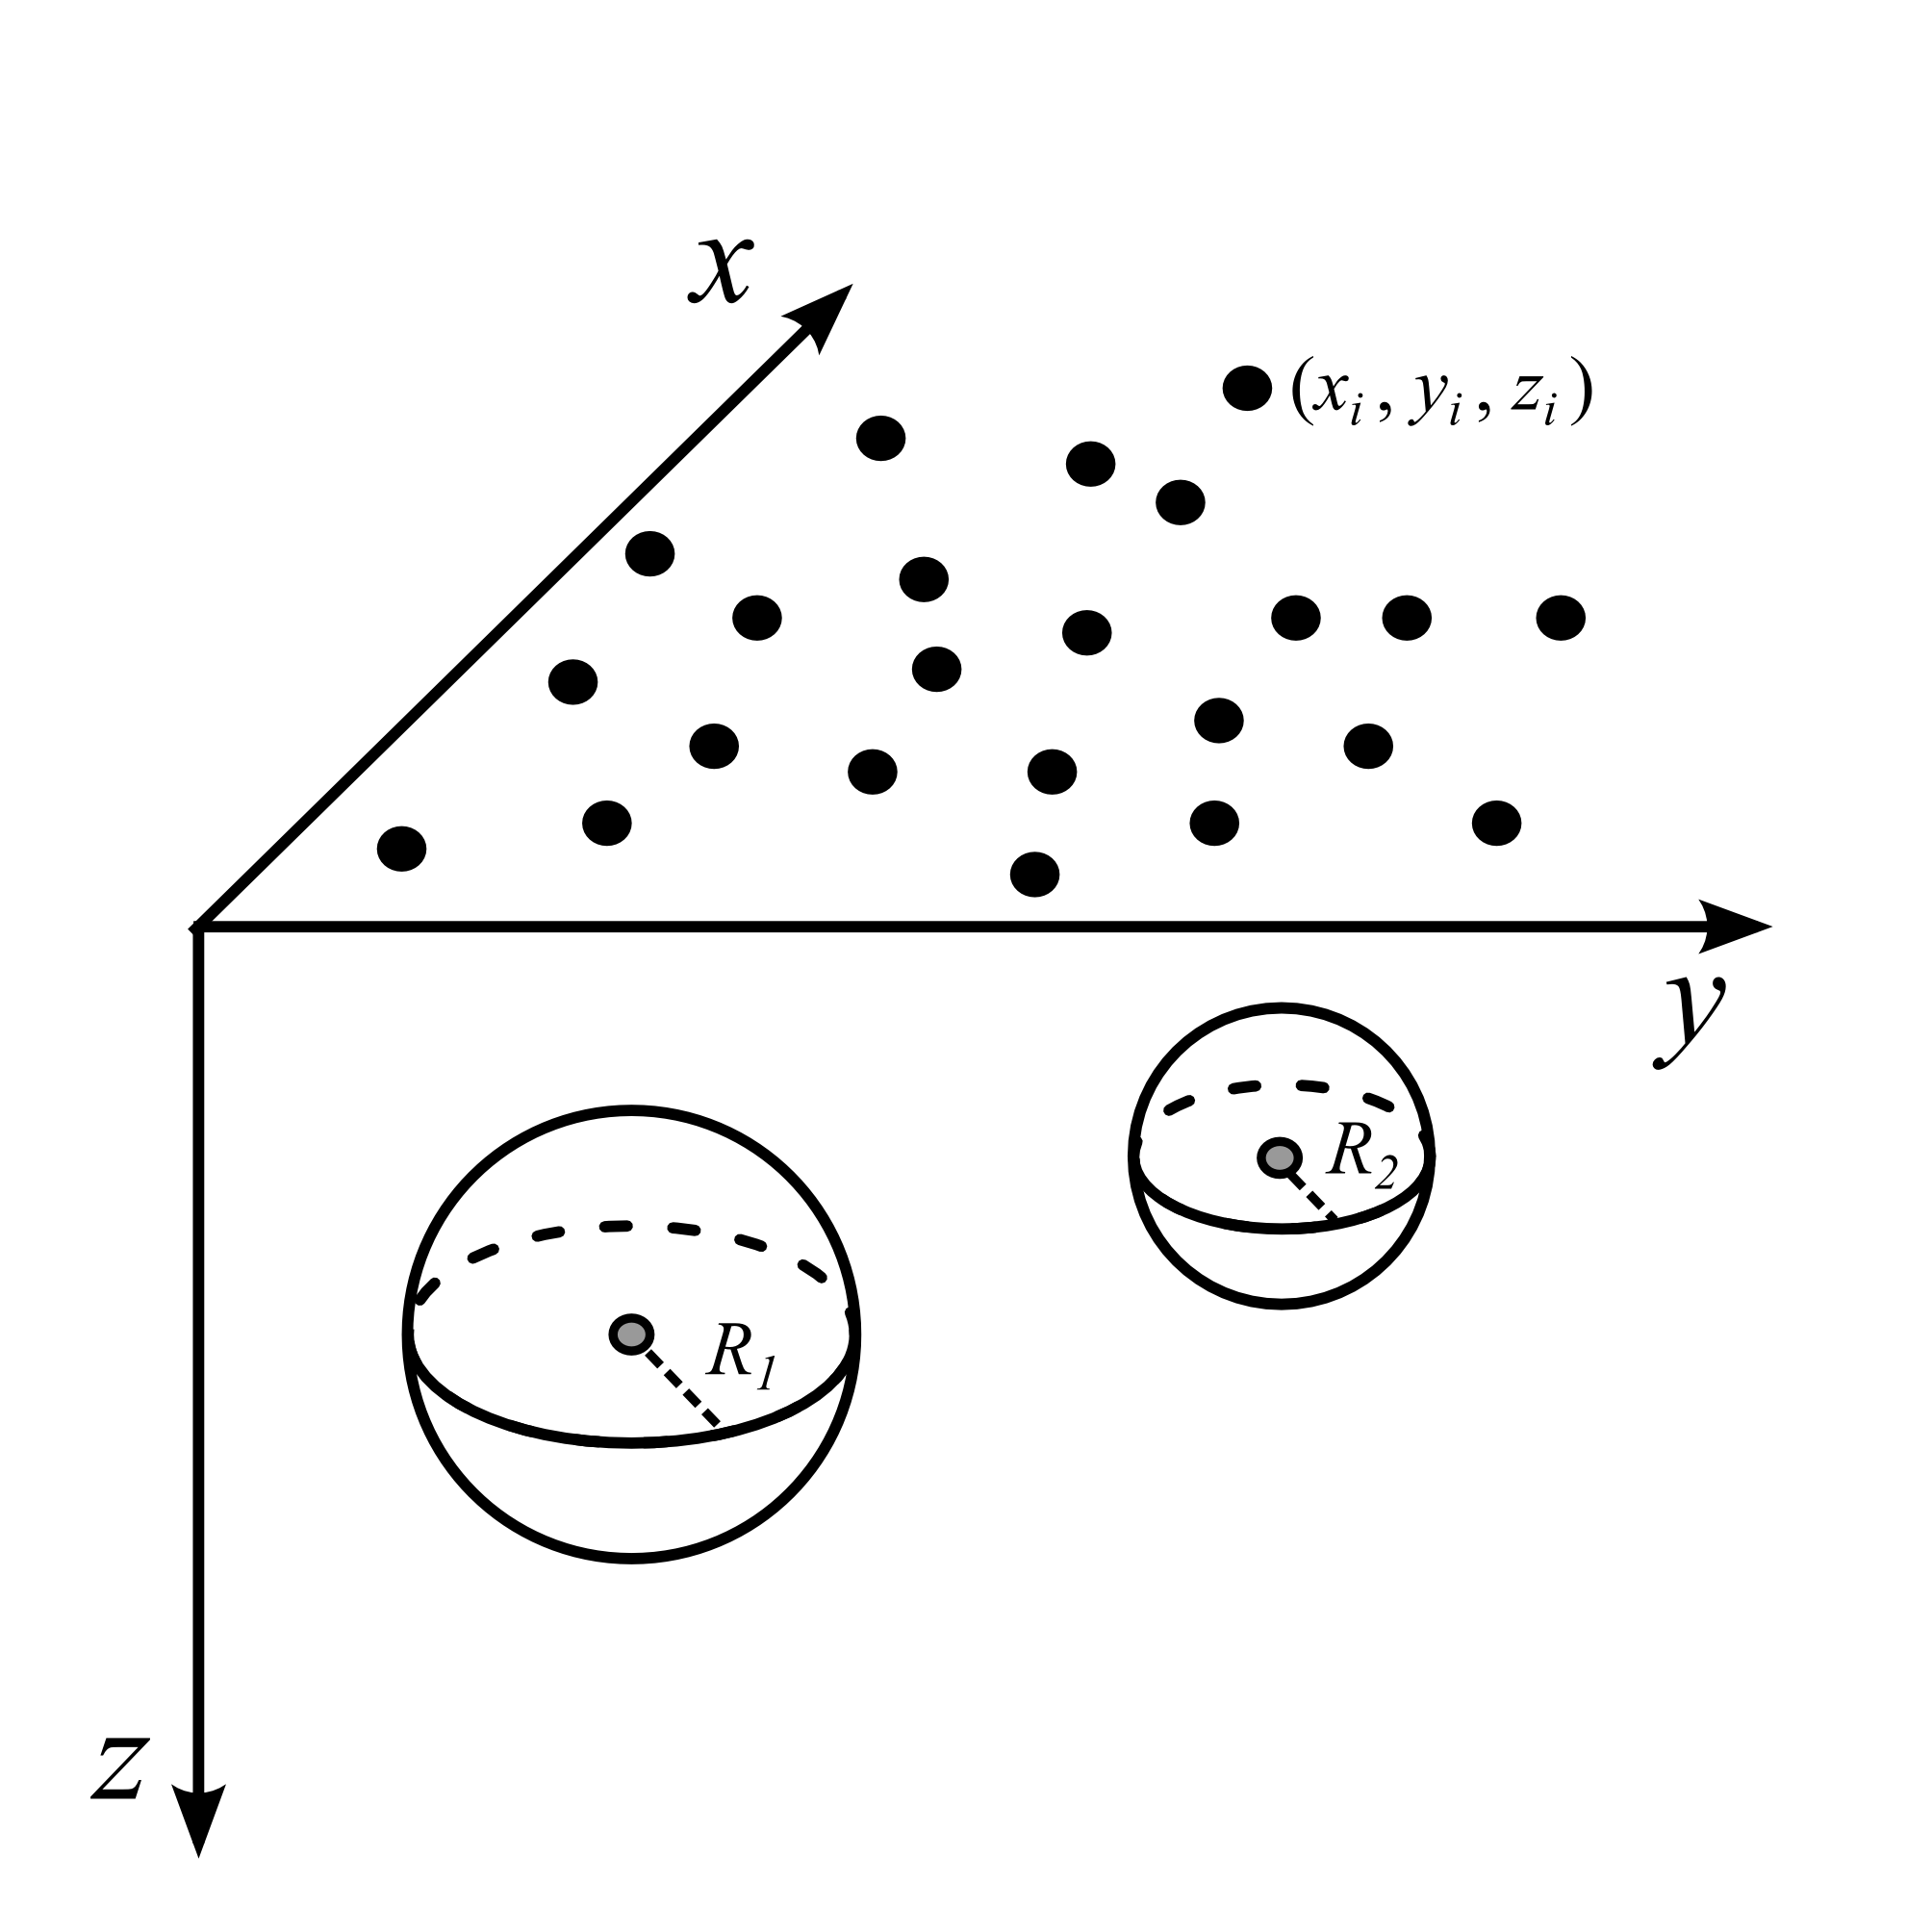
\includegraphics[width=8.3cm]{Figures/Fig1.png}
\end{center}
\caption{Schematic representation of $L = 2$ spheres uniformly magnetized at the subsurface. These spheres have radii $R_{j}$ (dashed straight lines), constant magnetization vectors $\vec{m}^{j}$ and centres (grey dots) at $(xc_{j}, yc_{j}, zc_{j})$, $j = 1, ..., L$. The total field anomaly produced by these spheres can be observed at the points $(x_{i}, y_{i}, z_{i})$, $i = 1, ..., N$ (black dots). In this Cartesian coordinate system, $x$ points to the geographic North, $y$ points to East and $z$ points downward.}
\label{fig:geometric-aspects}
\end{figure}

\begin{figure}[t]
\vspace*{2mm}
\begin{center}
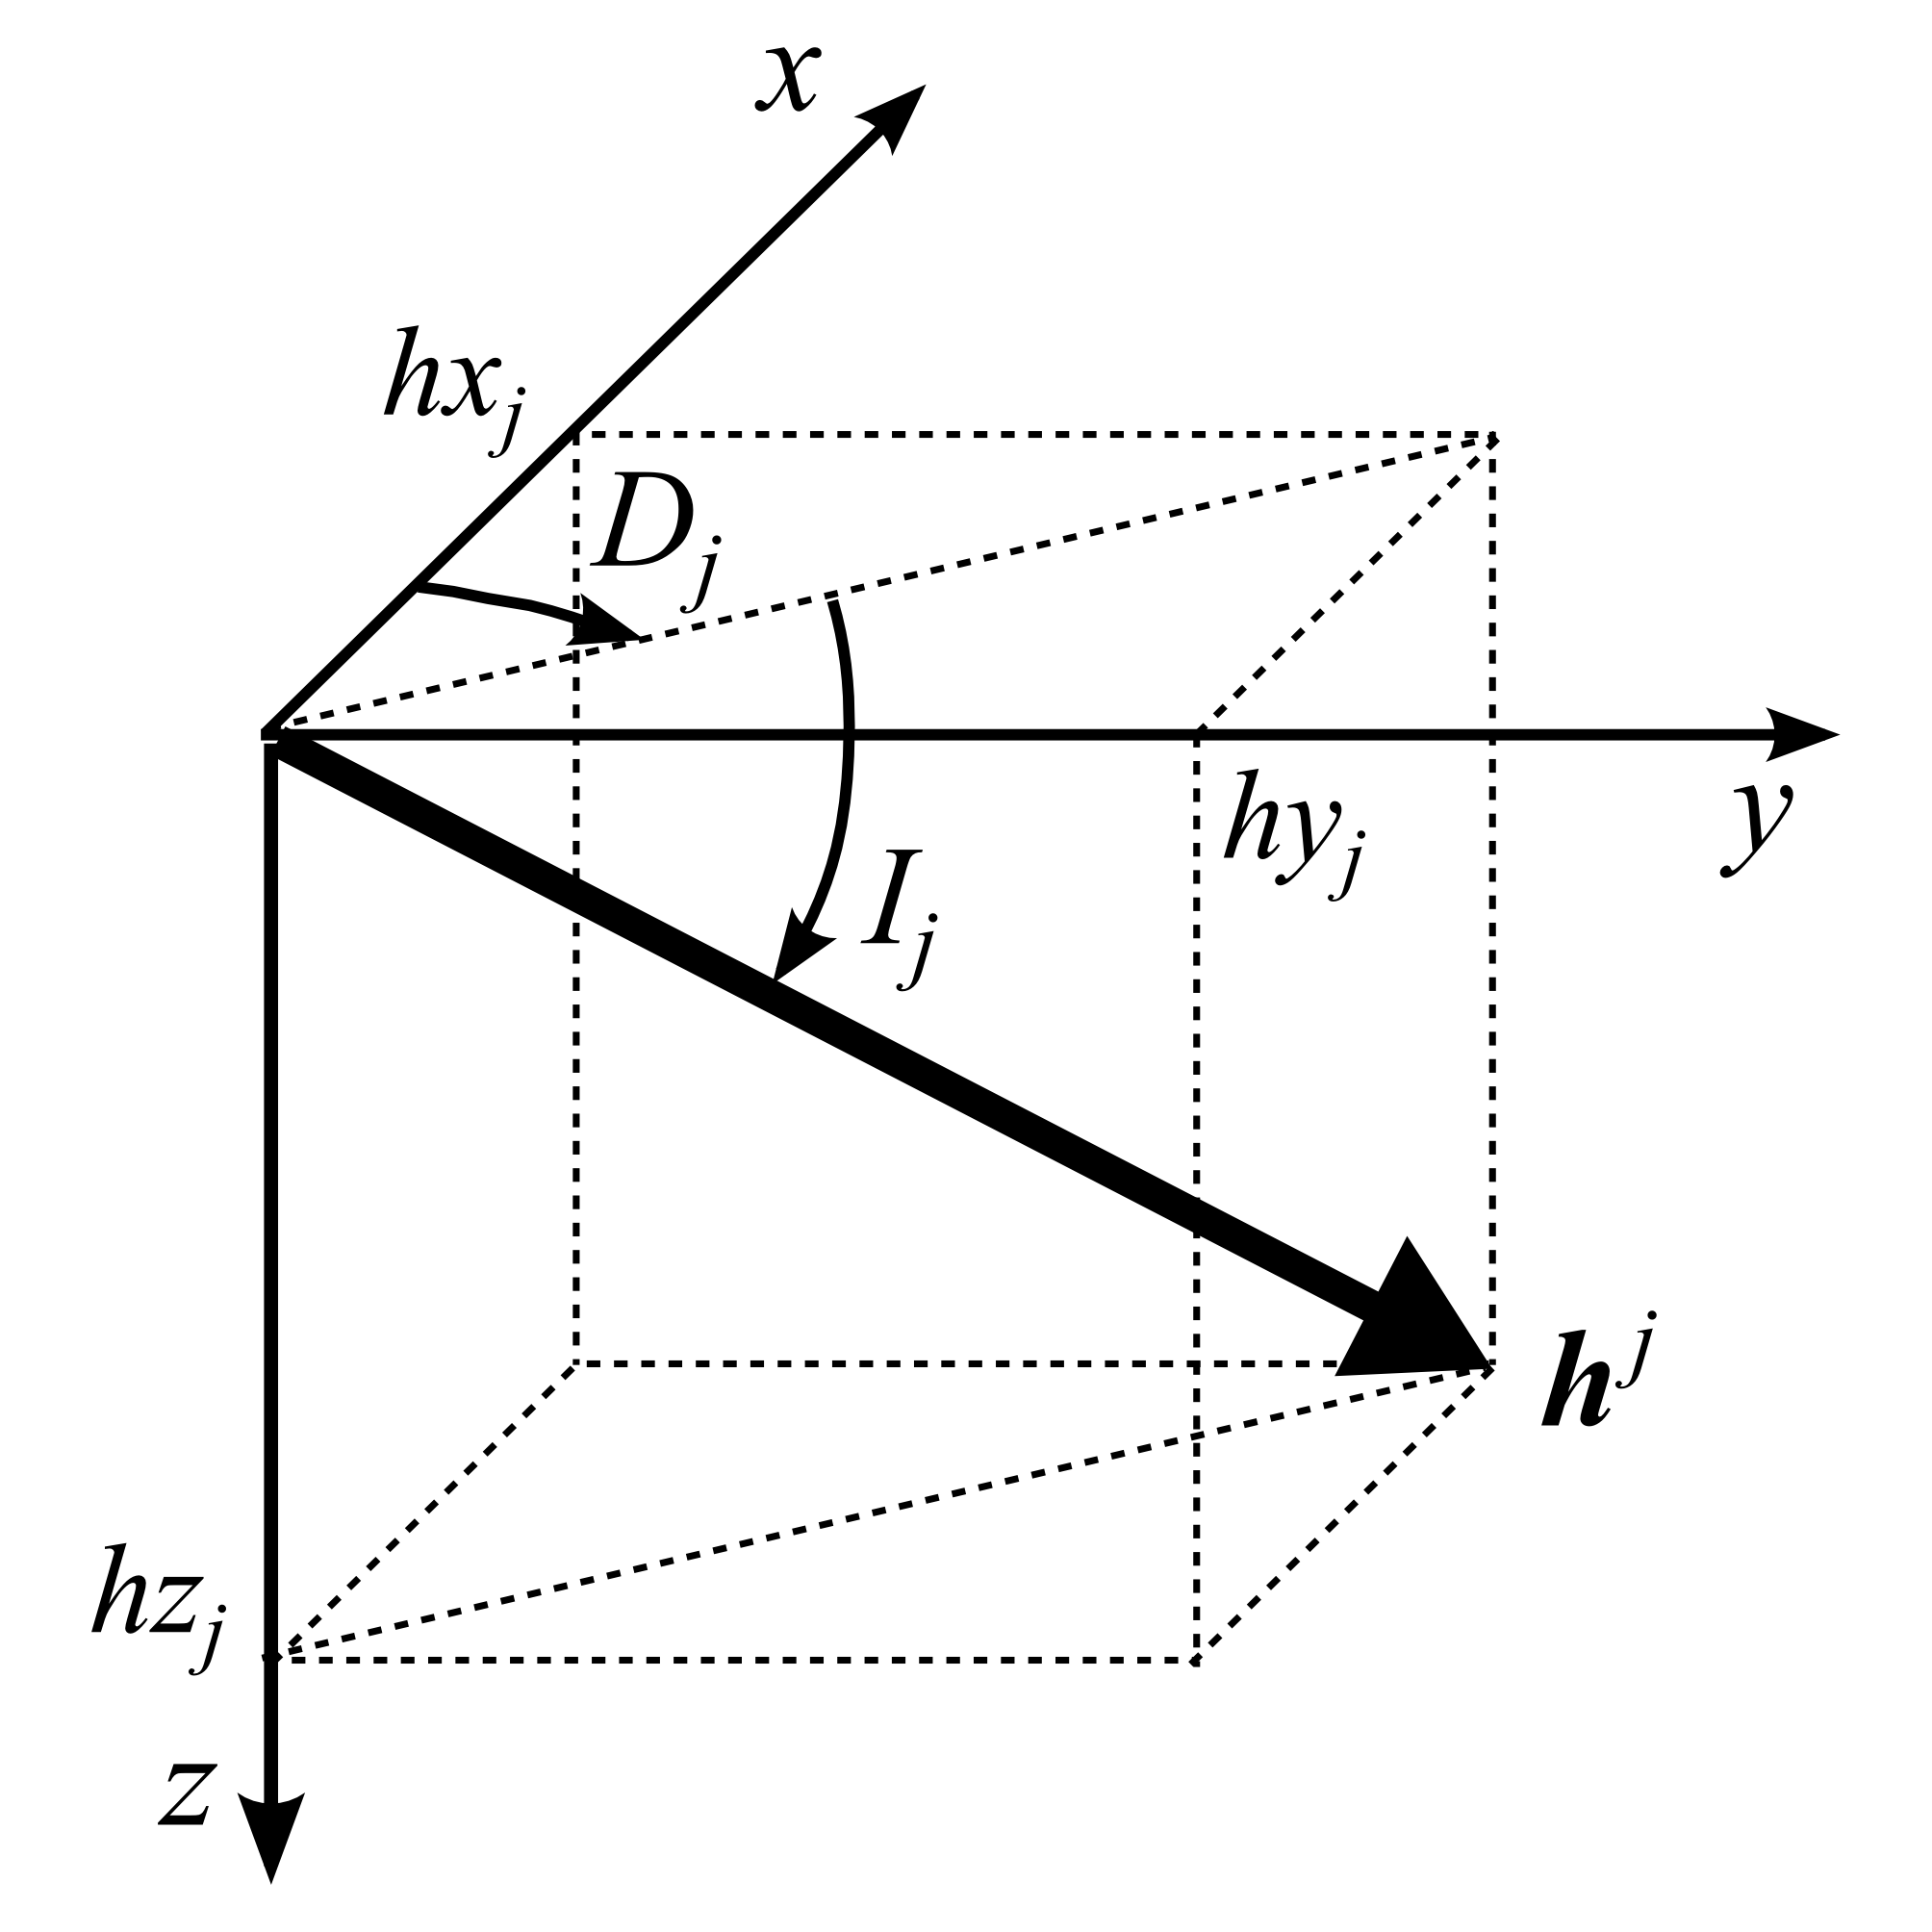
\includegraphics[width=8.3cm]{Figures/Fig2.png}
\end{center}
\caption{Schematic representation of the vector $\vec{h}^{j}$ (Eq. \ref{eq:hj}) with elements $hx_{j}$, $hy_{j}$ and $hz_{j}$ described in Cartesian coordinates. This vector has a declination $D_{j}$ (positive from $x$ to $y$) and inclination $I_{j}$ (positive downward), $j = 1, ..., L$.}
\label{fig:spherical-coordinates}
\end{figure}

%% TWO-COLUMN FIGURES

%f
%%\begin{figure*}[t]
%%\vspace*{2mm}
%%\begin{center}
%%\includegraphics[width=12cm]{FILE NAME}
%%\end{center}
%%\caption{TEXT}
%%\end{figure*}


%% TABLES %%%%%%%%%%%%%%%%%%%%%%%%%%%%%%%%%%%%%%%%%%%%%%%%%%%%%%%%%%%%%%%%%%%%


%% ONE-COLUMN TABLE

%t
%%\begin{table}[t]
%%\caption{TEXT}
%%\vskip4mm
%%\centering
%%\begin{tabular}{column = lcr}
%%\tophline
%%
%%\middlehline
%%
%%\bottomhline
%%\end{tabular}
%%\end{table}


%% TWO-COLUMN TABLE

%t
%%\begin{table*}[t]
%%\caption{TEXT}
%%\vskip4mm
%%\centering
%%\begin{tabular}{column = lcr}
%%\tophline
%%
%%\middlehline
%%
%%\bottomhline
%%\end{tabular}
%%\end{table*}


%% The different columns must be seperated with a & command and should
%% end with \\ to identify the column brake.

%%%%%%%%%%%%%%%%%%%%%%%%%%%%%%%%%%%%%%%%%%%%%%%%%%%%%%%%%%%%%%%%%%%%%%%%%%%%%%


%% If figures and tables must be numbered 1a, 1b, etc. the following command
%% should be inserted before the begin{} command.

\addtocounter{figure}{-1}\renewcommand{\thefigure}{\arabic{figure}a}


\end{document}
